% This file is iccc.tex.  It contains the formatting instructions for and acts as a template for submissions to ICCC.  It borrows liberally from the AAAI and IJCAI formats and instructions.  It uses the files iccc.sty, iccc.bst and iccc.bib, the first two of which also borrow liberally from the same sources. The format has been updated for the ICCC2022 to include a new, mandatory section to be included in camera-ready manuscripts.


\documentclass[letterpaper]{article}
\usepackage{iccc}


\usepackage{times}
\usepackage{helvet}
\usepackage{courier}
\usepackage{amsmath}
\usepackage{musicography}
\usepackage{graphicx}
\usepackage[font=small,skip=4pt]{caption}

\pdfinfo{
/Title (Formatting Instructions for Authors)
/Subject (Proceedings of ICCC)
/Author (ICCC)}
% The file iccc.sty is the style file for ICCC proceedings.
%
\title{Converting DNA to Music: Sonifying Splicing and Translation}
\author{Ilana Shapiro\\
Computer Science Department\\
Pomona College\\
Claremont, CA 91711 USA\\
issa2018@mymail.pomona.edu\\
}
\setcounter{secnumdepth}{0}

\begin{document} 
\maketitle
\begin{abstract}
The sonification of genetic material is a little-explored mode of unconventional computation that bridges the divide between bioinformatics, computer science, and music, allowing bioinformaticians to perceptualize their data in a novel and illuminating manner. This paper presents BioMus, an original model for converting DNA to musical data in the form of MIDI piano chords. Gene sequences are sourced from Ensembl, a genome database of the European Bioinformatics Institute, and are parsed into exons and and introns. Exons are further parsed into their 5' and 3' untranslated regions (UTRs) and their CDS (CoDing Sequence, i.e. the spliced exons constituting the amino acid-coding sequence after UTRs are removed). Then, each codon in the CDS is mapped to a major chord based on the amino acid it codes for, individual nucleobases in introns are mapped to diminished chords, and individual nucleobases in UTRs are mapped to minor chords. Rhythmic alterations indicate when CDS codons are broken across splice sites. To further emphasize protein-coding regions, all CDS chords are also at a higher volume. By mapping nucleobases and codons to chords and analyzing genetic material as music, BioMus thus gives scientists a novel and straightforward means to conceptualize the process of biological splicing and translation.

ONE PARAGRAPH, max 250words
\end{abstract}

\section{Introduction}

\section{Related Work}

Ingalls et al. present 

\section{Background}
Genes consist of sequences of DNA. The double-stranded DNA helix is shaped like a ladder, where each rung consists of two complementary nucleotides paired together. Every nucleotide is built on a $nucleobase$, which in DNA are adenine (A), cytosine (C), guanine (G) and thymine (T), and have the complementary pairings C-G and A-T. The DNA helix consists of the \textit{coding strand} and the \textit{template strand}. The template strand codes for mRNA during $transcription$, where each nucleotide is converted to its complement, and thymine is replaced with the base uracil.% https://www.khanacademy.org/science/ap-biology/gene-expression-and-regulation/transcription-and-rna-processing/a/overview-of-transcription
Subsequently, mRNA is converted to amino acids (the building blocks of proteins) during $translation$. Every gene codes for a single protein.

Transcription in eukaryotes includes a stage called \textit{RNA splicing}, where certain regions called $introns$ are removed, or ``spliced out," from the original DNA sequence. The final ``mature" mRNA solely consists of the remaining regions, called exons, that are connected to each other. The exons comprising mature mRNA consist of two \textit{untranslated regions}, or UTRs, and the \textit{CoDing Sequence}, or CDS. 

The CDS is a sequence of nucleotides that corresponds with the sequence of amino acids in a protein during translation. It begins with the start codon (ATG) and terminates with a stop codon (TAA, TAG, or TGA). In the CDS, nucleotides grouped into three to create $codons$. Each codon codes for a single amino acid. The UTR preceding the CDS is called the \textit{5' UTR}, and the UTR following the CDS is called the \textit{3' UTR}.

Note that in the original pre-transcription DNA sequence, both the UTRs and the CDS may be spread across multiple exons (i.e. they may be broken into multiple sections by intervening introns). In the CDS, this means that individual codons may be broken across splice sites: the codon will begin at the end of one exon, and conclude at the beginning of the next exon.

Figure \ref{fig:gene} shows the splicing process for a sample gene. 

\begin{figure}[h!]
\centering
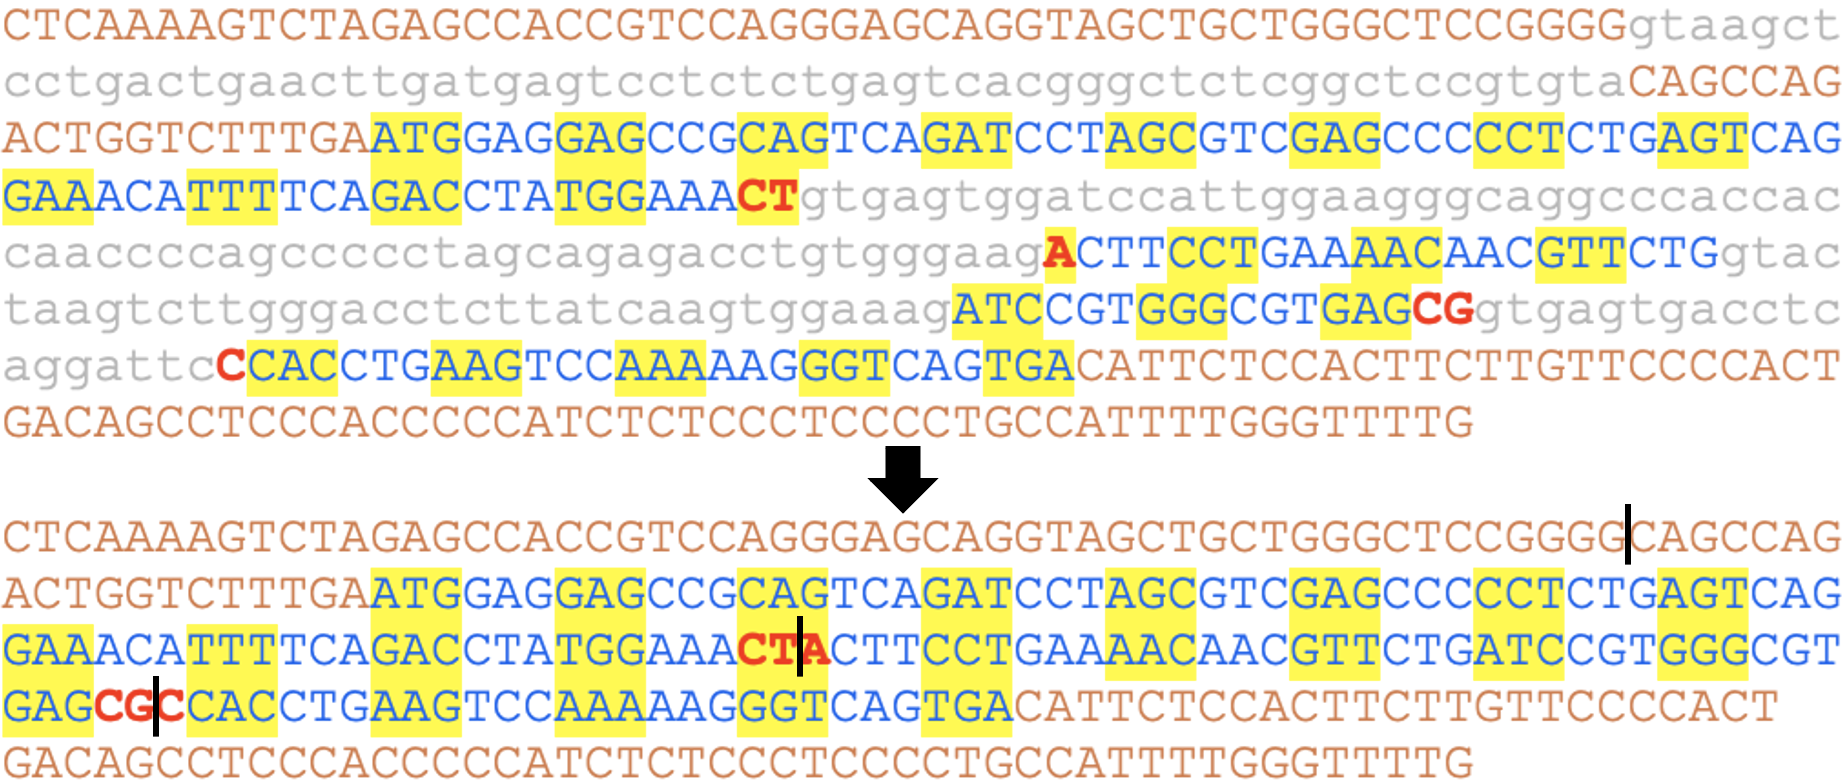
\includegraphics[width=0.48\textwidth]{images/gene.png}
  \caption{Homo sapiens}\label{fig:gene}
  \vspace{-3mm}
\end{figure}

The top sequence in Figure \ref{fig:gene} presents the gene before transcription, and the bottom sequence presents the result of splicing represented with \textit{complementary DNA}, or cDNA. A cDNA sequence is complementary to its source mRNA sequence and contains thymine rather than uracil; it is identical to the template DNA strand without the introns. Biologists synthetically construct cDNA from mRNA as a more convenient way to work with the sequence.

In Figure \ref{fig:gene}, exons are in color with capitalized nucleobase, while introns are lowercase and gray. The UTRs are in orange, and the CDS is in blue and red. Red nucleobases in the CDS indicate codons that are broken across splice sites. Notice how the 5' UTR is broken across the first two two exons, and the CDS is broken across the final four exons. In the CDS, codons are explicated by the alternating highlights. After we have spliced the introns from the gene, we end up with the contiguous sequence of exons in the bottom sequence in Figure \ref{fig:gene}. Splice sites are indicated with the black vertical bars.

\section{Converting DNA to Music}
\subsection{Obtaining Genetic Data}
BioMus's process of DNA sonification begins with the user specifying a desired species and gene. This information is passed to Ensembl's REST API to obtain Ensembl's choromomal coordinates of the gene's exons. These coordinates are sourced from the gene's \textit{canonical transcript}, the gene's transcript in Ensembl that is overall the most conserved and highly expressed, has the longest CDS, and is also represented in other major databases such as the NCBI \cite{ensembl_transcript_flags}. The exon coordinates also define the chromosomal coordinates of the intervening introns. Each pair of exon and intron coordinates is passed back to the Ensembl REST API to obtain the nucleobase sequences for each region, and the result is a list of alternating exons and introns. For instance, consider the abbreviated sequence obtained from Ensembl for the \textit{Homo sapiens} (human) TP53 tumor suppressor gene in Figure \ref{fig:pre_processed_seq_homo_sapiens_tp53}. Ellipses indicate omitted nucleobases for the sake of example.

\begin{figure}[h!]
\centering
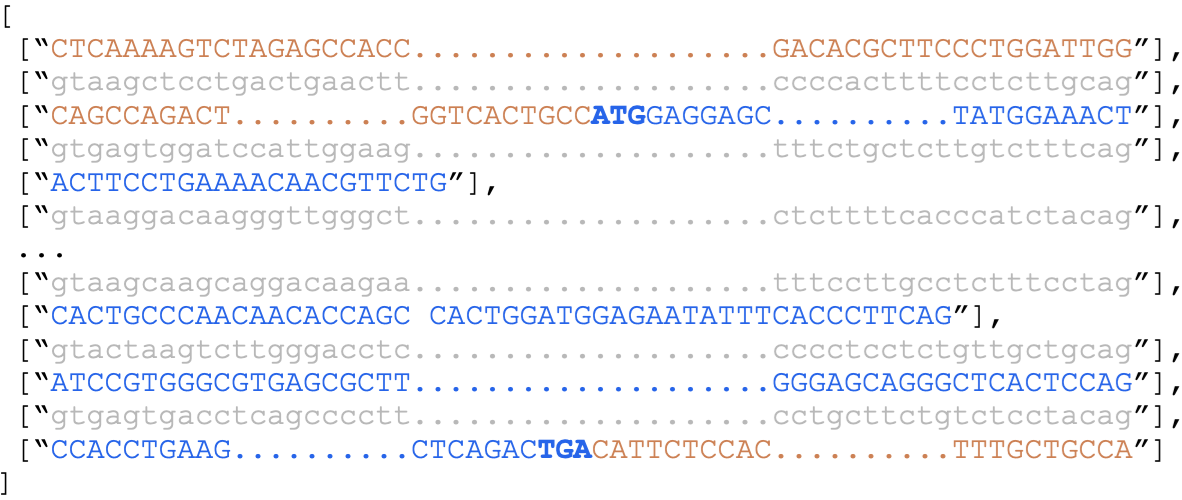
\includegraphics[width=0.48\textwidth]{images/pre_processed_seq_homo_sapiens_tp53_ABBREV}
  \caption{Homo sapiens}\label{fig:pre_processed_seq_homo_sapiens_tp53}
  \vspace{-3mm}
\end{figure}

Exons are in color, while introns are in grey. Within the exons, the orange regions are the UTRs, and the blue regions are the CDS. Notice how the CDS begins with the bolded start codon ATG and ends with the bolded stop codon TGA. 

Now, the goal is to extract the 5' UTR from the list. In order to ensure the correct CDS, is necessary to verify the 5' UTR with Ensemble, since it may include multiple ATG start codons that do not signal the start of the CDS. This is not necessary for the 3' UTR, since once we know we are in the CDS, the first stop codon will always signal the end of the CDS and the beginning of the 3' UTR. We obtain the 5' UTR from Ensembl by querying the Ensembl REST API for the cDNA sequence of the canonical transcript. By requesting Ensembl to ``mask" the UTRs of the cDNA sequence by representing them in lowercase, we can successfully isolate the 5' UTR and extract it from the list in Figure \ref{fig:pre_processed_seq_homo_sapiens_tp53}. As seen in Figure \ref{fig:post_processed_seq_homo_sapiens_tp53}, we end up with a list of the 5' UTR regions (top), and a list of the CDS regions and introns (bottom).\cite{10.1162/artl_a_00325}

\begin{figure}[h!]
\centering
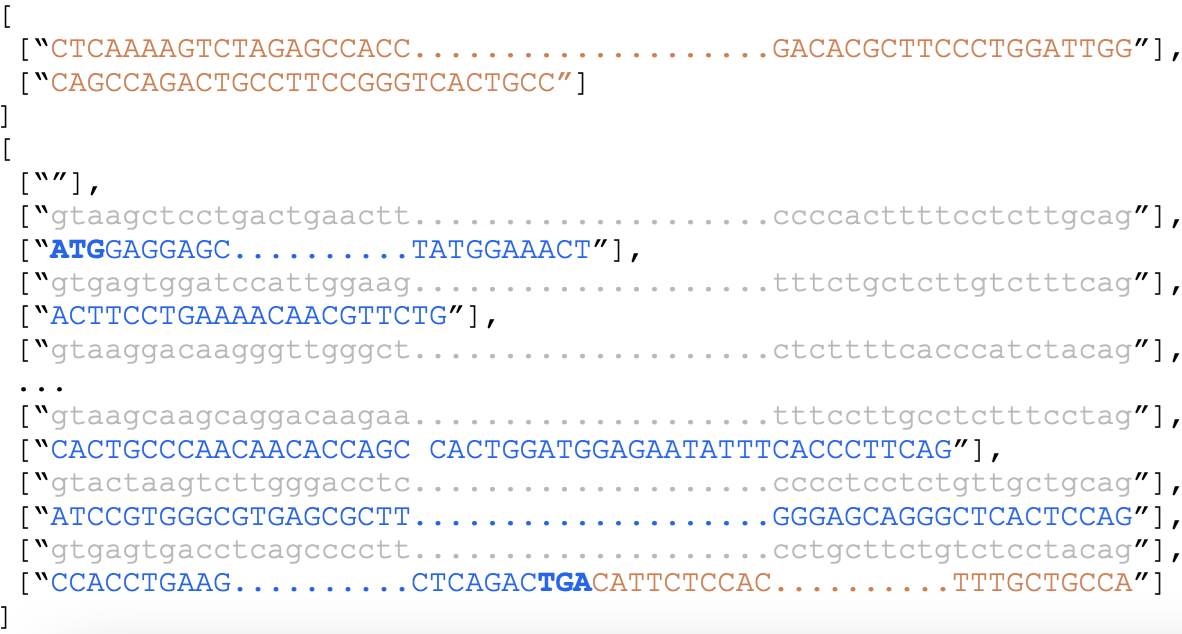
\includegraphics[width=0.48\textwidth]{images/post_processed_seq_homo_sapiens_tp53_ABBREV}
\vspace{-3mm}
  \caption{Homo sapiens}\label{fig:post_processed_seq_homo_sapiens_tp53}
  \vspace{-3mm}
\end{figure}

We now have all the tools necessary to translate the genetic data into music.

\subsection{Conversion to MIDI}

MIDI conversion begins by using the MIDIUtil Python library to create a MIDI track with the tempo set to \musQuarter\;= 200 BPM. Subsequently, individual nucleobases in UTRs are mapped to minor dyads (two-note chords), codons in the CDS are mapped to major triads, and individual nucleobases in introns are mapped diminished triads. 

Sonification of the gene begins with the 5' UTR, and the initial key is set to C minor. No key changes occur in UTRs or introns; the key is exclusively changed in the CDS and is determined by the codon. Thus, before the CDS begins, all introns and the 5' UTR remain in the initial key of C minor. After the CDS begins, the key of an intron is determined by the final codon in the preceding exon (whether or not that codon is broken across the splice site). The stop codon terminating the CDS then determines the key of all subsequent introns as well as the 3' UTR.

To construct the minor dyads in the 5' and 3' UTRs, BioMus defines the following mapping of individual nucleobases to musical notes relative to the local musical key in Table  \ref{table:nucleobases}.

\begin{table}[h!]
\centering
\begin{tabular}{|l|l|}
\hline
C   & Tonic    \\ \hline
G,A & Mediant  \\ \hline
T   & Dominant \\ \hline
\end{tabular}
\caption{DNA Base Mappings}
\label{table:nucleobases}
\end{table}

The minor dyad corresponding to each nucleobase in a UTR is constructed with its base pair using the mapping in Table  \ref{table:nucleobases}. For instance, if the key is C minor and we encounter the nucleobase C or G, then the dyad will consist of the notes C (tonic) and E\musFlat \; (mediant). Similarly, if we encounter the nucleobase A or T, then the dyad is E\musFlat \; and G (dominant). All UTR dyads are represented with quarter notes.

To construct the diminished triads in introns, BioMus again uses the mapping of individual nucleobases to musical notes in Table  \ref{table:nucleobases}. Initially, a minor dyad is constructed as in the UTRs. However, here we also add the diminished seventh scale degree from the local key to each dyad to construct the diminished triads. For instance, if the key is C minor and we encounter the nucleobase C or G, then the triad will consist of the notes C (tonic), E\musFlat \; (mediant), and B\musDoubleFlat (diminished seventh). Similarly, if we encounter the nucleobase A or T, then the triad will consist of the notes E\musFlat, G (dominant), and B\musDoubleFlat. We use the term ``diminished triad" loosely here, since technically only the latter triad described fits the formal definition of a diminished triad, with two minor thirds stacked on top of one another. However, as both chords outline a diminished seventh chord, their sonority is similar enough that we dub them both diminished triads as a way of distinguishing them from major or minor chords. Like UTRs, all intron triads are represented with quarter notes. 

When the CDS begins, we map codons (groups of three nucleobases), rather than individual nucleobases, to chords. The first codon in the CDS is always ATG, the start codon, which is mapped to a C major triad and is given a half note duration, rather than a quarter note, to signify the start of the protein-coding region. Subsequent chords return to quarter notes. To further emphasize we are in a protein-coding region, the volume is doubled throughout the CDS. The volume is halved to its original value whenever we encounter an intron, and doubled again when we return to the CDS in the next exon. 

We now want each amino acid encoded in the CDS to map to a unique chord. We thus want to create an injective mapping between amino acids and chords. We can do this by first solely considering the set of essential and nonessential amino acids (with which we can create a bijective mapping with the set of possible keys), and separately considering the set of conditionally essential amino acids (with which we can create an injective mapping with the set of possible keys).

Figures \ref{table:essential} and \ref{table:nonessential} explicate the chosen bijective mapping between the set of essential and nonessential amino acids and the set of possible keys. The codons that code for each amino acid are listed in the left hand column, and BioMus maps each to a major triad in the corresponding key in the right column. 

\begin{table}[h!]
\centering
\begin{tabular}{|l|l|l|}
\hline
ATG & \begin{tabular}[c]{@{}l@{}}Methionine/\\Start Codon\end{tabular} & C                         \\ \hline
ATT, ATC, ATA & Isoleucine                        & C\musSharp \\ \hline
AAA, AAG &  Lysine                      & D                         \\ \hline
ACT, ACC, ACA, ACG & Threonine                       & E\musFlat  \\ \hline
TTT, TTC & Phenylalanine                       & E                         \\ \hline
TGG & Tryptophan             & F                         \\ \hline
\begin{tabular}[c]{@{}l@{}}TTA, TTG, CTT, CTC, \\CTA, CTG\end{tabular}  & Leucine                       & F\musSharp \\ \hline
CAT, CAC & Histidine                       & G                         \\ \hline
GTT, GTC, GTA, GTG &  Valine                      & A\musFlat  \\ \hline
\end{tabular}
\caption{Essential Amino Acids}
\label{table:essential}
\end{table}

\begin{table}[h!]
\centering
\begin{tabular}{|l|l|l|}
\hline
AAT, AAC & Asparagine & A                        \\ \hline
GAT, GAC & Aspartate  & B\musFlat \\ \hline
GCT, GCC, GCA, GCG & Alanine    & B                        \\ \hline
\end{tabular}
\caption{Nonessential Amino Acids}
\label{table:nonessential}
\end{table}


Next, we consider the set of nonessential amino acids. Tables \ref{table:essential} and \ref{table:nonessential} explicate the chosen injective mapping between this set and the set of possible keys. Notice that the mapping is also bijective between the nonessential amino acids and the set of natural keys. 

\begin{table}[h!]
\centering
\begin{tabular}{|l|l|l|}
\hline
TAT, TAC & Tyrosine                & C \\ \hline
TGT, TGC & Cysteine                & D \\ \hline
\begin{tabular}[c]{@{}l@{}}TCC, TCT, TCA, TCG, \\ AGT,  AGC\end{tabular}  & Serine                  & E \\ \hline
\begin{tabular}[c]{@{}l@{}}AGA, AGG, CGT, CGC, \\ CGA, CGG\end{tabular}  & Arginine                & F \\ \hline
CCT,  CCC, CCA, CCG & Proline                 & G \\ \hline
CAA, CAG, GAA, GAG  & \begin{tabular}[c]{@{}l@{}}Glutamine/\\Glutamic acid\end{tabular}  & A \\ \hline
GGT, GGC, GGA, GGG & Glycine                 & B \\ \hline
\end{tabular}
\caption{Conditionally Essential Amino Acids}
\label{table:conditionally_essential}
\end{table}

This time, BioMus maps each codon to an augmented triad, rather than a major triad, in the corresponding key in the right column. 

Finally, we consider the stop codons, which do not code for amino acids and instead terminate the CDS. They are mapped to minor triads in the keys explicated in Table \ref{table:stop_codons}. 

\begin{table}[h!]
\centering
\begin{tabular}{|l|l|}
\hline
UAA & C \\ \hline
UAG & E \\ \hline
UGA & G \\ \hline
\end{tabular}
\caption{Stop Codons}
\label{table:stop_codons}
\end{table}

Each stop codon chord is given a half note duration and the volume is halved to signify the end of the protein-coding region. The subsequent minor dyads in the 3' UTR return to quarter notes. 

\section{Sample Music}

\section{Conclusion}
BioMus serves as a bridge between bioinformatics, computer science, and music by giving scientists the creative means to 


\section{Acknowledgments}

I am very grateful to Professor Zachary Dodds of Harvey Mudd College for his invaluable mentorship throughout this project.


\bibliographystyle{iccc}
\bibliography{iccc}


\end{document}
